%
% Annual Cognitive Science Conference
% Sample LaTeX Paper -- Proceedings Format
%

% Original : Ashwin Ram (ashwin@cc.gatech.edu)       04/01/1994
% Modified : Johanna Moore (jmoore@cs.pitt.edu)      03/17/1995
% Modified : David Noelle (noelle@ucsd.edu)          03/15/1996
% Modified : Pat Langley (langley@cs.stanford.edu)   01/26/1997
% Latex2e corrections by Ramin Charles Nakisa        01/28/1997
% Modified : Tina Eliassi-Rad (eliassi@cs.wisc.edu)  01/31/1998
% Modified : Trisha Yannuzzi (trisha@ircs.upenn.edu) 12/28/1999 (in process)
% Modified : Mary Ellen Foster (M.E.Foster@ed.ac.uk) 12/11/2000
% Modified : Ken Forbus                              01/23/2004
% Modified : Eli M. Silk (esilk@pitt.edu)            05/24/2005
% Modified : Niels Taatgen (taatgen@cmu.edu)         10/24/2006
% Modified : David Noelle (dnoelle@ucmerced.edu)     11/19/2014
% Modified : Roger Levy (rplevy@mit.edu)     12/31/2018



%% Change "letterpaper" in the following line to "a4paper" if you must.

\documentclass[10pt,letterpaper]{article}

\usepackage{cogsci}

\cogscifinalcopy

\usepackage{hyperref}
\usepackage{pslatex}
\usepackage{apacite}
\usepackage{float} % Roger Levy added this and changed figure/table
                   % placement to [H] for conformity to Word template,
                   % though floating tables and figures to top is
                   % still generally recommended!
\usepackage{graphicx}
%\usepackage[none]{hyphenat} % Sometimes it can be useful to turn off
%hyphenation for purposes such as spell checking of the resulting
%PDF. Uncomment this block to turn off hyphenation.

\setlength\titlebox{6.5cm}
% You can expand the titlebox if you need extra space
% to show all the authors. Please do not make the titlebox
% smaller than 4.5cm (the original size).
%%If you do, we reserve the right to require you to change it back in
%%the camera-ready version, which could interfere with the timely
%%appearance of your paper in the Proceedings.

\title{SUSTAIN captures category learning, recognition, and hippocampal activation
in a unidimensional vs information-integration task}

\author{{\large \bf Lenard Dome (lenard.dome@plymouth.ac.uk)} \\
  School of Psychology, University of Plymouth \\
  Plymouth,  PL4 8AA UK
  \AND{\large \bf Charlotte E. R. Edmunds (ceredmunds@gmail.com)} \\
  Queen Mary, University of London \\
  London, E1 4NS UK
  \AND{\large \bf Andy J. Wills (andy.wills@plymouth.ac.uk)} \\
  School of Psychology, University of Plymouth \\
  Plymouth, PL4 8AA UK}


\begin{document}

\maketitle

\begin{abstract}
There is a growing interest in alternative explanations to the dual-system
account of how people learn category structures varying in their optimal
decision bounds (unidimensional and information-integration structures).
Recognition memory performance and hippocampal activation patterns in these
tasks are two interesting findings, which have not been formally explained.
Here, we carry out a formal simulation with SUSTAIN~\cite{Love2004}, an
adaptive model of category learning, which had great success in accounting
for recognition memory performance and fMRI activity patterns. We show,
for the first time, that a formal single-system model of
category learning can accommodate recognition performance after learning and
is consistent with fMRI data obtained while participants learned these
structures.

\textbf{Keywords:}
categorization; recognition memory; formal model; SUSTAIN
\end{abstract}

\section{Introduction}

One commonly used pair of category structures in categorization research are
the unidimensional (UD) and information-integration (II) category structures.
UD and II structures were initially used for trying to separate the
perceptual processes encoding the visual
information from the decision processes assigning a category response to the
perceptual effects~\cite{ashby1988decision}. Figure~\ref{fig:structures} shows
how stimuli varying in size and brightness are distributed within these two
category structures on either side of the boundaries. UD category structures
have a either vertical or horizontal decision bound: if the square
is darker or larger than the set threshold, then it is category A, otherwise it is category B.
Figure~\ref{fig:structures}A and~\ref{fig:structures}B shows that this optimal decision
bound is parallel to one of the dimensional axes in the physical stimuli space.
II structures are defined by diagonal optimal decision bounds.
Figure~\ref{fig:structures}C and~\ref{fig:structures}D shows that II decision bounds follow a linear
function, where the gradient is neither zero, nor infinite.

Many experiments utilised these structures~\cite<e.g.>{Carpenter2016,
Donkin2015, Nomura2007, le2019deferred} and  many initial empirical results
were taken as evidence for COVIS~\cite<COmpetition between Verbal and Implicit
Systems>{Ashby2011} --- one formalization of a
dual-system theory of categorization. Traditionally, dual-system theories
have two distinct architectures using functionally different mechanisms. In
COVIS, the explicit system uses rules that can be easily verbalized, while the
implicit system maps perceptual input onto category responses. Accuracy in UD
and II category structures, according to COVIS, depends on which system is
engaged in solving the task. COVIS predicts that the explicit system will
implement rules to optimally solve UD tasks, whereas the implicit system
will take charge if simple rules are inadequate and implements (in this case)
multidimensional strategies to combine information from the two dimensions
of II tasks.

However, results from multiple labs pointed out flaws in the experimental
designs in COVIS-inspired experiments~\cite{newell2013} with potential
alternative explanations~\cite{le2019deferred, Donkin2015}
or problems with the decision-bound analyses applied~\cite{edmunds2018a,
edmunds2019}. In turn, some of these alternative-to-COVIS explanations have been
critiqued~\cite{ashby2019dissociations}. The debate continues.

The current paper further examines some of the alternative-to-COVIS explanations
of how people classifiy II and UD structures. Specifically, the way COVIS explains
how people should optimally learn II structures was also
questioned by \citeA{Carpenter2016} and \citeA{3edmunds2016a}, who
provided direct evidence for an involvement of similar processes
in both II and UD problems.

\citeA{Carpenter2016} found that the medial temporal lobe (MTL) and specifically
the hippocampus (HPC) were more active when people were learning about
II structures compared to when they were learning about UD structures. This result
contradicts to predictions of COVIS as it is currently formalized, which posits
less activation for II than UD. COVIS states that the explicit system is mapped
to neurobiological substrates such as the MTL (HPC) and predominantly the
prefrontal cortex, while the implicit system is mapeed to areas such as the
supplementary motor areas and substantia nigra~\cite{ashby2017multiple}.
According to COVIS, HPC and the prefrontal cortex is exclusively involved in the
explicit system, which is responsible for the optimal learning of UD structures.
In other words, the way the two architectures are specified
in COVIS are inconsistent with the differences in activations
observed in HPC. HPC has also been long identified as crucial for
memory~\cite{oreilly2001, schlichting2015}.
and thought to be essential for explicit memory. This suggest that people
should have better recognition performance after learning II structures than
in UD structures.

Given~\citeA{Carpenter2016}'s observation of greater HPC activity in II than
in UD structures, one can further predict, contrary to COVIS, that there will
be better post-recognition memory for exemplars in II than in UD structures.
~\citeA{3edmunds2016a} directly confirmed this prediction.
They found better recognition memory after learning II than UD structures,
essentially supplementing the neural data. While the differences in
recognition performance are rather small, it is statistically present in
a between-groups comparison~\cite{edmunds2016}. A more extensive investigation
on recognition memory in UD and II problems also found that
participants who reported using complex multidimensional rules showed
better recognition performance~\cite{edmunds2017critique}.

Building on these findings, we further supplement behavioral and neural data
with evidence from computational modeling. Here, we provide a formal
single-system explanation of the results of both~\citeA{Carpenter2016}
and~\citeA{3edmunds2016a}. We do so by using SUSTAIN
~\cite<Supervised and Unsupervised STratified Adaptive Incremental
Network>{Love2004}.

SUSTAIN is one model in a single-system approach to modeling categorization, and
is able to accommodate a wide range of behavioral and neural
phenomena~\cite<e.g.>{Love2004, Gureckis2004, Davis2012a}. This breadth is
particularly admirable, because modelers tend to focus on a small subset
of effects~\cite{Wills:2017ez}.

There are two reasons for using SUSTAIN. First, SUSTAIN
can accommodate recognition memory performance in multiple tasks~\cite{Love2007,
Davis2012a, mack2018}. Second, SUSTAIN's concept-forming and -altering mechanism,
adaptive clustering, has been mapped to HPC and MTL functions and
activations.

Cluster-specific model components in SUSTAIN have been directly
connected to strong HPC activations present in early learning and low HPC
functions in amnesic patients in a dot-pattern classification task~\cite<for a more exhaustive review, see>{Love2007}.
SUSTAIN views the hippocampus as the constructor and editor of clusters ---
binding information together into category representations,
and views the MTL familiarity signals as indicators of cluster re-activations.
These views have been reinforced by connecting computational
modeling to neural activity patterns. For example, during rule-plus-exception
learning, SUSTAIN makes specific predictions about item recognition, which
has been directly and consistently mapped to MTL activations
~\cite{Davis2012a}. Furthermore, SUSTAIN's cluster-updating mechanism parallels
HPC activity in response to changing task demands. SUSTAIN accommodates
behavioral responses and HPC activity in subsequent learning tasks where the
stimuli remain perceptually the same, but irrelevant features
in the first task become essential in the new categorization problem~\cite{mack2016}.
SUSTAIN is well matched with how the HPC binds together information into
meaningful category representations and updates the stored representations
to match with goal-oriented changes in task-demands~\cite<for a complete review,
see>{mack2018}.

More difficult tasks require SUSTAIN to bind (and store) larger sets of
information into clusters than simpler tasks do~\cite{Love2004}. This process
results in higher number of clusters being recruited, which has been previously
mapped to increased HPC activity and improved recognition accuracy~\cite{Love2007}.
SUSTAIN therefore predicts better recognition performance in tasks that
require higher number of clusters. In this paper, we intend to test these
predictions in relation to UD and II category structures by formally fitting
SUSTAIN to the categorization accuracy data
of~\citeA{3edmunds2016a}. Furthermore, we will compare its recognition performance
to human recognition performance from~\citeA{3edmunds2016a}
and evaluate whether the cluster-recruitment process is consistent with increased
HPC activity in II problems compared to UD problems observed in~\citeA{Carpenter2016}.

\begin{figure}[h]
    \centering
    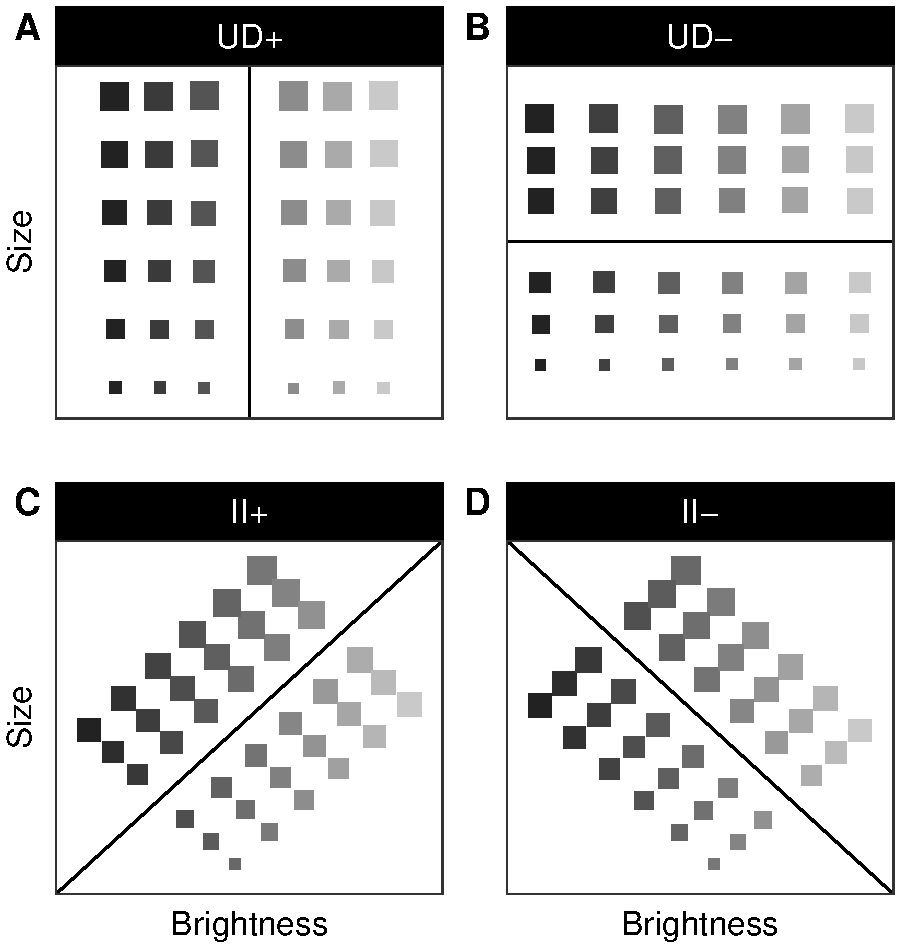
\includegraphics[width=8cm,
  height=10cm,
  keepaspectratio,]{pdf/categoryStructures.pdf}
  \caption{Representations of the category structures used in Edmunds et al. (2016).
    UD = unidimensional; II = information-integration; +/- = vertical/horizontal
    for UD and positive/negative for II.}
   \label{fig:structures}
\end{figure}

We refer the reader to \citeA{Love2004} for the full description of the
model's architecture and \citeA{Love2007} for the full description of the
supplementing architecture capturing recognition memory.

Briefly, SUSTAIN is an adaptive clustering model, which proposes that clusters
underlie category representations~\cite{Love2004}. Clusters, from SUSTAIN's
perspective, are single coordinates in the representation space. These
coordinates are internal representations that connect to categories.
SUSTAIN starts with one
cluster, centered on the first input representation it encounters by default.
When SUSTAIN encounters a stimulus, it computes similarity from all stored
cluster representations in the psychological space. First, the distance is
calculated for each dimension, then differentially weighted
in the cluster activation function by attentional tunings.
So similarity on dimensions with higher attentional tunings will be more
impactful on which cluster is activated. The winning cluster will be the one
with the highest activation. After this algorithm, clusters are laterally
inhibited by each others' activations. Laterally inhibited activations are
considered to reflect the models' overall familiarity with the current stimulus.
The sum of these activations, Recognition score $R$, indexes this stimulus-specific
familiarity. Lateral inhibition then ends in a winner-takes-all fashion ---
non-winning clusters' activations are muted for calculating further response
probabilities.

Activations after lateral inhibition spread to the category output units
by weighted connections. The activations of each output units are
turned into response probabilities. If the model made the correct response, then
the winning cluster's position is adjusted by moving it closer to the current
input representation. In the event of a prediction error (an incorrect response)
a new cluster centered on the current input representation is recruited
and becomes the winning cluster. Connection weights from cluster units
to the category output units are updated according to the one-layer
delta learning rule \cite{widrow1960adaptive}.
After both correct and erroneous responses,
the winning cluster updates SUSTAIN's attentional tuning. Attentional tuning
of each dimension maximizes its impact on the recruited clusters.
SUSTAIN prefers simple solutions, and only starts recruiting clusters in
response to prediction errors. This means that more difficult tasks will
cause SUSTAIN to densely populate the psychological space with clusters.

\section{Simulation of Edmunds et al. (2016)}

In the following, we present a formal simulation with the SUSTAIN model
accommodating human categorization accuracy in II and UD structures.
In addition, we show how the model captures categorization accuracy
and predicts better recognition memory following the II problems compared to
the UD problems~\cite{3edmunds2016a}. This difference should be based on
more clusters recruited for II, which leads to the prediction of higher
hippocampal activation while learning the II structures compared to
UD structures~\cite{Carpenter2016}. We do so by fitting SUSTAIN to an abstract design
of \citeA{3edmunds2016a}. We decided on~\citeA{3edmunds2016a}, because
this allowed us to present the model with a close approximation of the conditions
present where the authors observed better recognition performance in II.

\citeA{3edmunds2016a} used 36 grey squares that varied in brightness and
size\footnote{In our simulations, these values were put in a range $[0, 1]$ within each
dimension. The values as specified by their respective coordinates are available in
the supplementary material}. There were four conditions. UD structures included
both vertical and horizontal category boundaries, shown on Figure~\ref{fig:structures}A
and Figure~\ref{fig:structures}B respectively. II structures involved diagonal category boundaries with
both positive and negative gradients, shown on Figure~\ref{fig:structures}C
and Figure~\ref{fig:structures}D respectively.

Each condition consisted of three phases. First, the categorization training
phase included 360 supervised training trials in blocks of 120. Each
simulated participant received 24 stimuli randomly picked from the 36 for their
simulation. Those 24 stimuli were shown 5 times in each of the 3 blocks.
This was followed by an OLD/NEW recognition phase. This phase
consisted of 3 blocks of all 36 stimuli. The last phase was
a categorization test phase. This phase was similarly made up of 3 blocks of
all 36 items. For a more detailed description of experimental
procedure, see \citeA{3edmunds2016a}.

\subsection{Simulation}

Our implementation of SUSTAIN is available in the R package
catlearn~\cite{wills2020}. First, we wanted to find the one best fitting
parameter set for the model across all four categorization problems. SUSTAIN
therefore encountered all four problems at the same time as a single participant
- SUSTAIN completed each problem once with the same set of parameters. SUSTAIN
was reset between each problem.
SUSTAIN's parameters were then adjusted to minimise the sum of squared errors (SSE).
SSE was calculated between the mean group-level accuracy of humans in the
categorization test phase
(as reported in Edmunds et al. (2006) and shown in Table~\ref{tab:accuracy})
and the mean accuracy of SUSTAIN during the
categorization test phase. We used the group-level data, because it
captures the ordinal difference associated with these tasks: participants
show higher accuracy for UD than II. The trial order was randomised on each iteration.
The model was fitted with a differential evolutionary algorithm, as implemented
in the DEoptim package~\cite{DEoptim}. The algorithm iterated
1000 times to find the best fitting parameters. The speed of crossover
was set to $c = 0.5$, which gave larger weights to successful
mutations. The top 30\% best solutions were copied to the new iteration and
was used in the new mutated population.
These settings helped to find the single overall best set of parameters
for all category structures across different trial orders. The best fitting
parameters are presented in Table~\ref{tab:parameters}.
After finding the best set of parameter, we simulated 1000 different
trial orders with SUSTAIN.

\begin{table}[h]

\caption{\label{tab:parameters}Best fitting parameters for SUSTAIN rounded to the
4\textsuperscript{th} decimal place.}
\centering
\begin{tabular}[t]{lc}
\hline
Parameters & Best Fitting \\
\hline
Attentional focus ($r$) & 4.1301 \\
Lateral inhibition ($\beta$) & 8.3273 \\
Decision consistency ($d$) & 1.9883 \\
Learning rate ($\eta$) & 0.0626 \\
\hline
\end{tabular}
\end{table}


\subsubsection{Categorization Test Phase Accuracy}

SUSTAIN's categorization performance is qualitatively similar to what we
observed from humans --- II structures are harder to learn than UD
in~\citeA{3edmunds2016a}.
This difference in accuracy is a reliable difference in SUSTAIN's performance,
$BF = 1.88 \times 10^{776}$.
SUSTAIN matches human-level categorization test performance with a mean
difference of 0.014, see Table~\ref{tab:accuracy}.

\begin{table}[H]
\caption{\label{tab:accuracy} Categorization accuracy in SUSTAIN and humans.
Standard deviations are in parenthesis.}
\centering
\begin{tabular}[t]{lcc}
\hline
Category Structures & SUSTAIN & Human \\
\hline
II & 0.78 (0.027) & 0.78 (0.11) \\
UD & 0.85 (0.026) & 0.87 (0.07) \\
\hline
\end{tabular}
\end{table}

\subsubsection{Cluster Recruitment and Attentional Tuning}

The mean number of clusters recruited were $M_{ii} = 5.59$,
$SD_{ii} = 1.20$ for II and $M_{ud} = 3.01$,
$SD_{ud} = 1.18$ for UD. SUSTAIN solves II with a minimum of 4
clusters and a maximum of 12 clusters. SUSTAIN solves UD with a minimum
of 2 and a maximum of 12 clusters. Example clusters populating the
psychological space are shown in Figure~\ref{fig:clusters}.

\begin{figure}[h]
    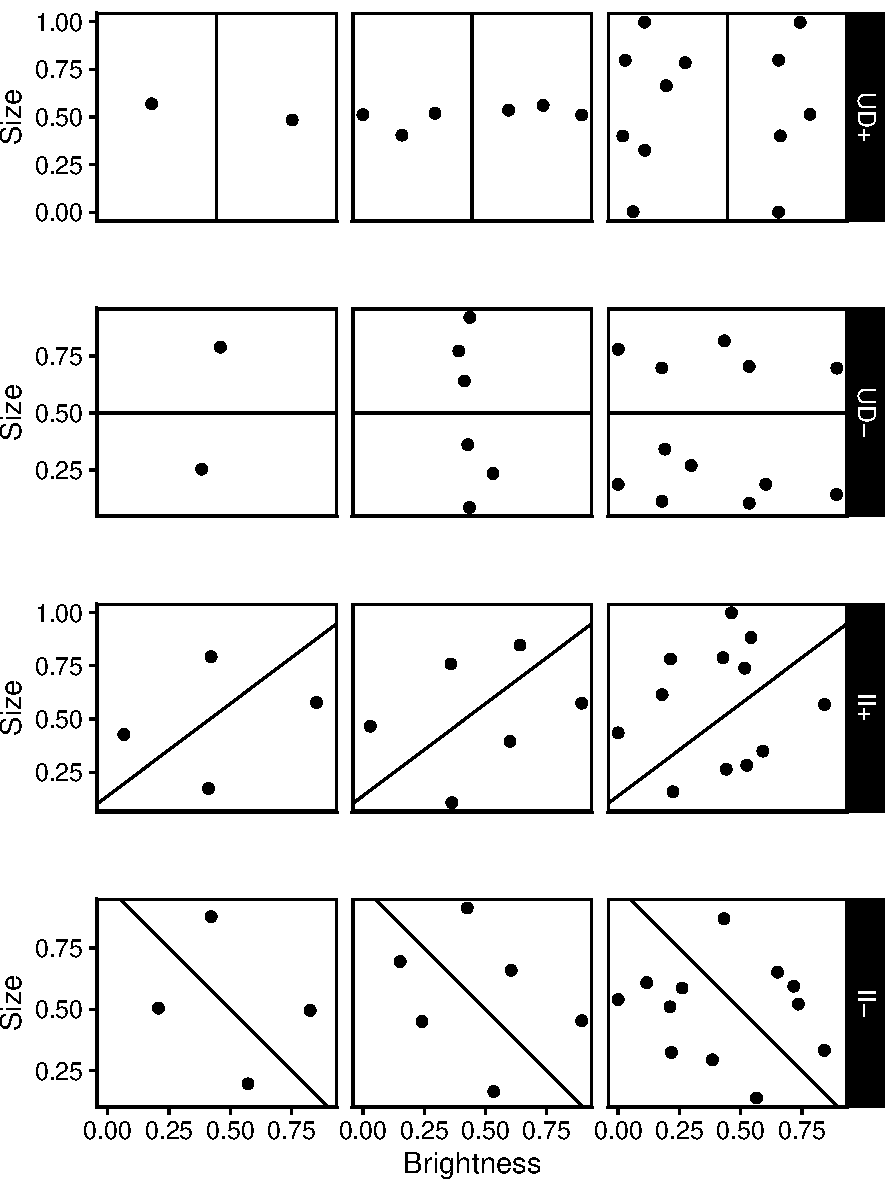
\includegraphics[width=12cm,
  height=11cm,
  keepaspectratio]{pdf/clusters_old_bw.pdf}
    \caption{Example clusters recruited by SUSTAIN for three simulations
    across conditions. The juxtaposed black lines are
    the optimal decision bounds. UD = unidimensional; II = information-integration;
    +/- = vertical/horizontal for UD and positive/negative for II.}
\label{fig:clusters}
\end{figure}

The mean, and variation, in the number of clusters is the consequence of
how trial-order interacts with
the following mechanisms: similarity, attention and error-driven
cluster recruitment.
Simple problems on average result in fewer clusters, while harder
problems require the recruitment of more clusters.
This is attenuated by differentially weighing in relevant information
from each dimension --- by attentional tuning of perceptual inputs.
Each dimension has its own attentional tuning, $\lambda$. For example,
$\lambda$ is higher for relevant dimensions in UD structures, but
remains comparable across dimensions in II, see Table~\ref{tab:lambda}.

\begin{table}[h]
    \centering
\caption{\label{tab:lambda}Mean $\lambda$ values for each dimension across
    all category structures. UD = unidimensional; II =
    information-integration; +/- = vertical/horizontal for UD and
    positive/negative for II. Standard deviations are in parenthesis.}
    \begin{tabular}[t]{ccc}
    \hline
    Conditions & $\lambda_{x}$ & $\lambda_{y}$ \\
    \hline
    II+ & 13.52 (0.81) & 13.46 (0.78) \\
    II- & 13.47 (0.78) & 13.51 (0.81)  \\
    UD+ & 13.38 (1.48) & 7.80 (1.41)  \\
    UD- & 7.80 (1.41) & 13.39 (1.48) \\
    \hline
    \end{tabular}
\end{table}

If SUSTAIN tries to incorporate the irrelevant dimension in UD by
attending to both dimensions equally, the only way SUSTAIN can eventually
solve the task is to recruit more clusters. Similarly, if SUSTAIN only attends
to a single dimension in II, it will need to recruit large number of clusters
to solve the task. This will also result in misclassification during the
categorization test phase. Figure~\ref{fig:clusters-stim} shows how the 36
stimuli are captured by different clusters (indicated by the dots' color) during
the categorization test phase. Figure~\ref{fig:clusters-stim} second row
gives an example when clusters from one side of the optimal decision
bound captures stimuli from the other side of the decision bound. This is due
to a single dimension weighting in more in cluster activations than the other
dimension.

% \begin{table}[H]

\caption{\label{tab:clusters}Summary statistics for the number of clusters
recruited by SUSTAIN.}
\centering
\begin{tabular}[t]{lcccc}
\hline
Category Structures & Mean & SD & Max & Min\\
\hline
II & 5.591 & 1.189 & 12 & 4\\
UD & 3.007 & 1.183 & 12 & 2\\
\hline
\end{tabular}
\end{table}


\begin{figure}[h]
    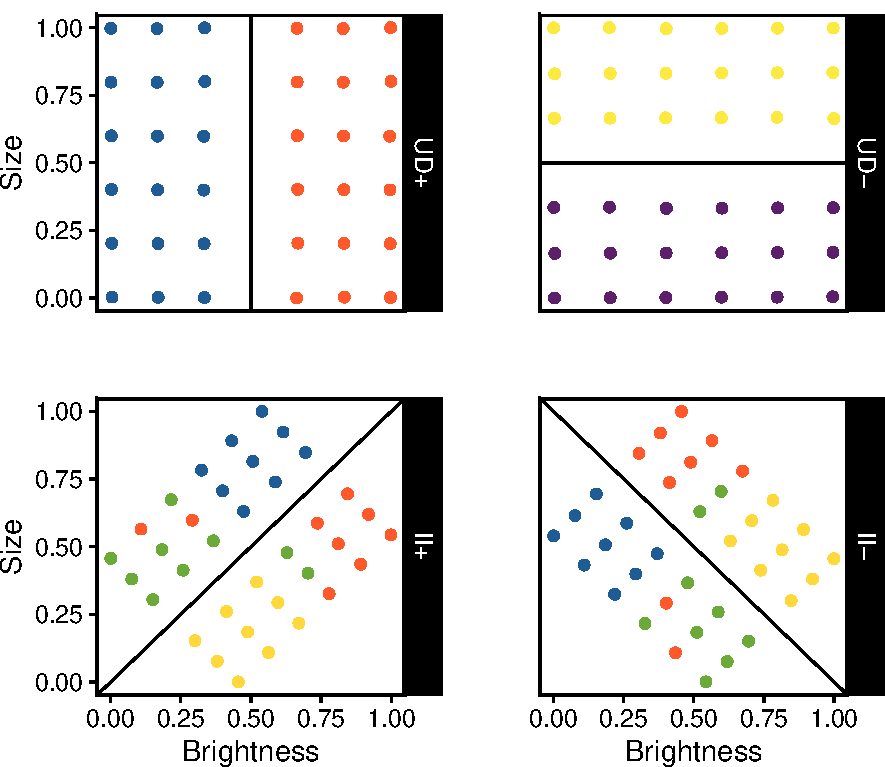
\includegraphics[width=8cm,
  height=10cm,
  keepaspectratio]{pdf/clusters_single.pdf}
    \caption{Example physical stimuli space for a single simulation during the
        categorization phase. Each color is a different cluster SUSTAIN recruited
        during learning. The dots
        with same colors are captured by the same cluster. The juxtaposed black lines are
    the optimal decision bounds. UD = unidimensional; II = information-integration;
    +/- = vertical/horizontal for UD and positive/negative for II.}
   \label{fig:clusters-stim}
\end{figure}

Overall, SUSTAIN requires higher numbers of clusters to solve II due to its
difficulty. This will result in clusters more perfectly matching training items,
so the matching clusters will dominate the activation function. From the model's
point of view, the HPC is specifically responsible for encoding new clusters
after surprising events~\cite{Love2007}. We see higher HPC activations in
II, because the category structure requires more representations to be encoded
by the HPC. HPC activations have been shown to positively relate to cluster
activations, updates and recruitments in SUSTAIN~\cite{mack2016, mack2018}.
Therefore, SUSTAIN's prediction for the difference in HPC activity between
UD and II problems is found to be consistent with~\citeA{Carpenter2016}.

\subsubsection{Recognition}

\begin{table}[h]

\caption{\label{tab:recognition}Mean recognition scores and d' for each category
    structure, rounded to three decimal places. Standard deviations are in
    parenthesis.}
\centering
\begin{tabular}[t]{lcc}
\hline
&  SUSTAIN $d'$ & Human $d'$\\
\hline
II & 0.040 (0.056) & 0.01 (0.02)\\
UD & -0.016 (0.135) & 0.00 (0.01)\\
\hline
\end{tabular}
\end{table}


To get an approximate $d'$ measure from $R$, Recognition Score, we applied
Equation A11 from \citeA{Love2007} to turn stimulus-specific $R$ values
during the categorization test phase into choice probabilities: $P(old) = R /\ (R + k)$
where $k$ is a response threshold parameter. We calculated the mean probability
of a hit $(P(H) = P(old \mid item_{old})$ and false alarm $P(F) = P(old \mid
item_{new})$ for each simulated participant. We continued to
determine $d'$ for each participant using the z-transformed $P(H)$ and $P(F)$.
Then we calculated group-level averages. This algorithm (including
the group-level $d'$ calculations) were fitted against human performance
in the recognition phase as indexed by $d'$. Similarly, we used DEoptim and
reitereted the paramater search 50 times. More details are included in the code
available in the supplementary material.

We found that the best-fitting parameter $k$
was $0.571$. This parameter will not change the ordinal pattern of the
recognition performance ($II > UD$) SUSTAIN shows given the simulated
categorization test data, but simply brings the values closer to the human data.

Table~\ref{tab:recognition} shows the performance of humans and SUSTAIN.
A comparison of d' between SUSTAIN and human data yields a mean difference of
$0.023$. The model predicts better recognition performance after learning II
than UD structures, consistent with~\citeA{3edmunds2016a}.
This is a realiable difference in the simulated data, BF = $7.06 \times 10^{57}$.
This difference of $d'$ between SUSTAIN's recognition performance in II and UD
results from the difference in the number of recruited clusters between the
two structures.

Recognition in SUSTAIN is based on similarity-driven cluster activation and
lateral inhibition. Where SUSTAIN recruits a large number of clusters, these
clusters will generally be closer to the stimulus representations presented
in the recognition memory test. This means that the stored
representions will match better to the model's previous experience in II than in
UD problems. The more densely populated the psychological space with clusters,
the more clusters neighbouring the input representation will activate. These
activations then compete and will diminish as a result of
lateral inhibition. The better recognition memory performance in II results
from the higher sum of activations in regions neighbouring the input representations.

This benefit parallels HPC activation patterns.
Better recognition memory performance follows not just from the modeling
perspective, but also from a neural point-of-view.
\citeA{Love2007} predicted this relationship, where higher number of
clusters mirror higher levels of HPC involvement. This prediction strongly
aligns with \citeA{Carpenter2016}, who observed higher HPC involvement in the
II compared to UD task, and our simulation, where SUSTAIN recruits more
clusters for the II task.

\section{Discussion}

We have presented a formal account of empirical results
\cite{3edmunds2016a, Carpenter2016}
concerning the acquisition of unidimensional (UD) and information-integration
(II) category structures. In so doing, we have shown - for the first time -
that both the behavioral and neuroimaging data obtained in these tasks can be
accomodated by a single-system model, SUSTAIN. The increased number of clusters
recruited by SUSTAIN for the II structure served as a base for better
recognition memory performance, and larger HPC activation, than in the UD
structure. According to SUSTAIN, this is because the differing task demands of
the two structures requires a larger amount of information to be encoded in
the HPC for II structures.

Previously,~\citeA{Davis2012a} speculated that tasks like the II category learning
were not suitable to model with SUSTAIN. This sentiment was based on the
idea that II category learning is a procedural learning task~\cite{Nomura2007}
--- and hence characterized by mechanisms not specified within SUSTAIN.
However, procedural accounts of II problems are based on a range of experiments
that received considerable scrutiny, and which turn out to have alternative
explanations.

While the findings reported here are preliminary,
they provide a sufficient explanation for a range of findings
related the UD and II structures in the form of a fully specified formal
computational model --- SUSTAIN. Nonetheless, our current simulation might
be considered unconstrained, because
we did not pursue quantiative fit per se. Instead we choose to focus
on whether SUSTAIN could accomodate the UD/II differences in performance during
the categorization test. We then investigated the predictions SUSTAIN made on that
basis relating to the subsequent recognition task, and the differences in MTL/HPC
activations across UD and II. One promising follow-up would be to
explore individual differences in HPC activations and categorization
accuracy via fitting SUSTAIN to subject-level results. This would allow
a direct mapping between cluster recruitment and HPC activations. A caveat with
this approach is SUSTAIN's sensitivity to trial-order effects.

The only formal model --- before SUSTAIN --- that has been argued to accomodate
the classification of both UD and II structures was COVIS. COVIS posited
a procedural account of how people learn II structures. COVIS solves II
with a procedural learning mechanism conceptualized as a three-layer network:
the first layer calculates the exponent
of the distance between activated input units and and sensory units;
the second layer attenuates these similarities by weighted connections
between sensory units and striatal units before spreading to the striatal units;
in the third layer, a decision rule responds with the most activated striatal unit;
and then the weights are updated.
It is a distributed-representation connectionist network, where input
node activations are supplied by a distance between sensory unit coordinates
and input representation in the psychological space. COVIS solves
UD by a different, rule-based system, which establishes a decision bound dominating responding.
Therefore, at limit COVIS predicts no recognition memory
for either category structures. This still doesn't allow better recognition
in II than UD. One approach
would be to create an architecture that converts similarity derived from
sensory input and weighted connections to activations of memory traces.
A similar approach has been used to describe recognition by multiple-trace
memory models~\cite{hintzman1986schema}, but this can require the assumption
that both rule-based and procedural
systems are able to access the representation space where these values are
stored.

\section{Conclusion}

We formally show that a single-system adaptive clustering model, SUSTAIN,
can accommodate categorization and recognition performance in two frequently
used category structures, information-integration and unidimensional.
The behavior of the model is also consistent with MTL and HPC activity involved
in learning these structures. Our simulation not only provides a formal
account of how people learn these structures, but also contributes to the
literature bridging formal models of category learning, behavior and the
brain.

\section{Open Science Statement}
All simulation code is available in the Open Sciences Framework at
\url{https://osf.io/jc9xs/}.

\bibliographystyle{apacite}

\setlength{\bibleftmargin}{.125in}
\setlength{\bibindent}{-\bibleftmargin}

\bibliography{pu037cogsci}

\end{document}
